\chapter{Integrating Learning and Planning}

The goal of this lecture is to provide as an introduction of \textit{learning a model} of an MDP directly from experience, and use \textit{planning} to construct a value function or policy. These two are then combined into a single architecture. The difference between Model-Free and Model-Based RL are the following:
\begin{itemize}
	\item Model-Free
	
	No model, learn value function (and/or policy) from experience
	\item Model-Based
	
	Learn model from experience, plan value function (and/or policy) from model
\end{itemize}

\section{Model-Based RL}

\begin{figure}[H]
	\centering
	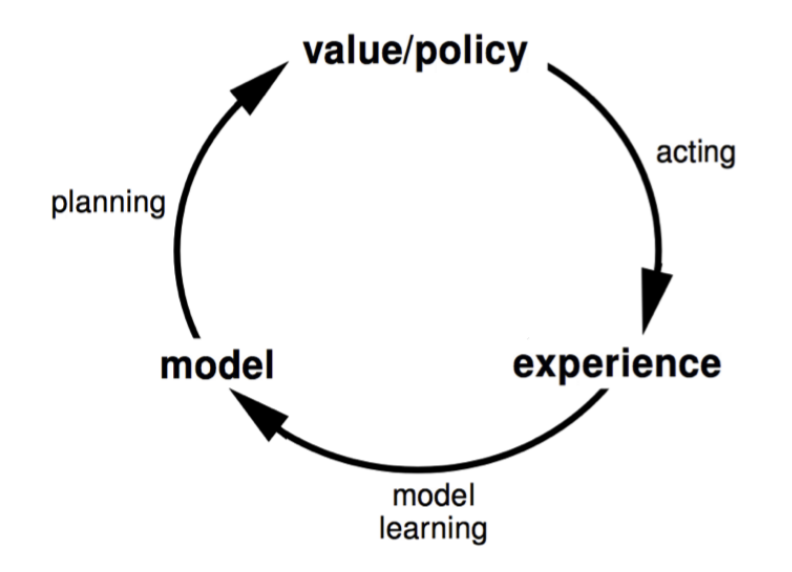
\includegraphics[width=6cm]{model-based-rl}
	\caption{Model-Based RL cycle}
\end{figure}

The advantages of Model-Based RL are that models can be efficiently learned using \textit{supervised learning} methods. It is also possible to then reason of model uncertainty. A disadvantage, however, is that first the model must be learned. Only then can the value function be constructed. This also means there are two sources of approximation error, and the accuracy of the value function is limited to the accuracy of the model.

A \textit{model} $M$ is a representation of an MDP parameterized by $\eta$. In this case, it is assumed that the state and action spaces are known (for simplification). So then, a model $M = (P_\eta, R_\eta)$ represents state transitions $P_\eta \approx P$ and rewards $R_\eta = R$. These can be used to estimate rewards and state transitions:

\begin{equation*}
	\begin{aligned}
		S_{t+1} & \sim P_\eta(S_{t+1} | S_t, A_t)\\
		R_{t+1} & = R_\eta(S_{t+1} | R_t, A_t)
	\end{aligned}
\end{equation*}

Typically, a conditional independence between state transitions and rewards are assumed ($P(S_{t+1}, R_{t+1} | S_t, A_t) = P(S_{t+1} | S_t, A_t)P(R_{t+1} | S_t, A_t)$).

So, the goal is to estimate $M_\eta$ from experience $\{S_1, A_1, R_2, ..., S_T\}$. This is a supervised learning problem. More specifically, it is usually best to split up the two tasks of learning $R_\eta$ and $P_\eta$. $S_t, A_t \Rightarrow R_{t+1}$ is a \textit{regression problem}, while $S_t, A_t \Rightarrow S_{t+1}$ is a \textit{density estimation} problem.

There are a lot of ways to create a model. This chapter focusses on the \textit{Table-Lookup Model}. 

\subsection{Table-Lookup Model}

The idea here is to count the visits $N(s, a)$ to each state-action pair. Then, similar to what TD learns, the idea is to construct the maximum-likelihood Markov model from this. It can be constructed in the following manner.

\begin{equation}
	\begin{aligned}
		& \hat{P^a_{ss'}} = \frac{1}{N(s,a)} \sum_{k = 1}^K \sum_{t = 1}^{T_k} 1(s^k_t, a^k_t, s^k_{t+1} = s, a, s')\\
		& \hat{R^a_{s}} = \frac{1}{N(s,a)} \sum_{k = 1}^K \sum_{t = 1}^{T_k} 1(s^k_t, a^k_t = s, a)r^k_t
	\end{aligned}
	\label{eq:sampling-from-model}
\end{equation}

Alternative, it is possible to record an experience tuple $(S_t, A_t, R_{t+1}, S_{t+1})$ at each time-step $t$. In order to then sample the model, uniformly randomly pick a tuple matching $(S_t, A_t, ., .)$.

\subsection{Planning with a Model}

Given a model $M_\eta = (P_\eta, R_\eta)$, the goal is to solve the MDP $(S, A, P_\eta, R_\eta)$ using a planning algorithm (e.g. Value iteration, Policy iteration, Tree search, ...).

Algorithms like Value iteration are quite expensive, since they go over the entire state(-action) space. \textbf{Sample-Based} planning uses the model to generate samples. This is often much more efficient. It also means more frequent states will be sampled more often. This can be a good property to have.

The sampling happens in the same way as in equation \ref{eq:sampling-from-model}. At each step, model-free RL can be applied to the samples (e.g. Monte-Carlo control, SARSA, Q-Learning, ...).

Given an imperfect model $(P_\eta, R_\eta) \neq (P, R)$, the performance of model-based RL is limited to the optimal policy of approximate MDP $(S, A, P_\eta, R_\eta)$. So, when the model is inaccurate, planning will compute a sub-optimal policy. It is always possible to switch to model-free RL. However, there are ways of reasoning about the \textit{uncertainty} in the model. This can be done using for example Bayesian modelling.


\section{Integrated Architectures}

\begin{figure}[H]
	\centering
	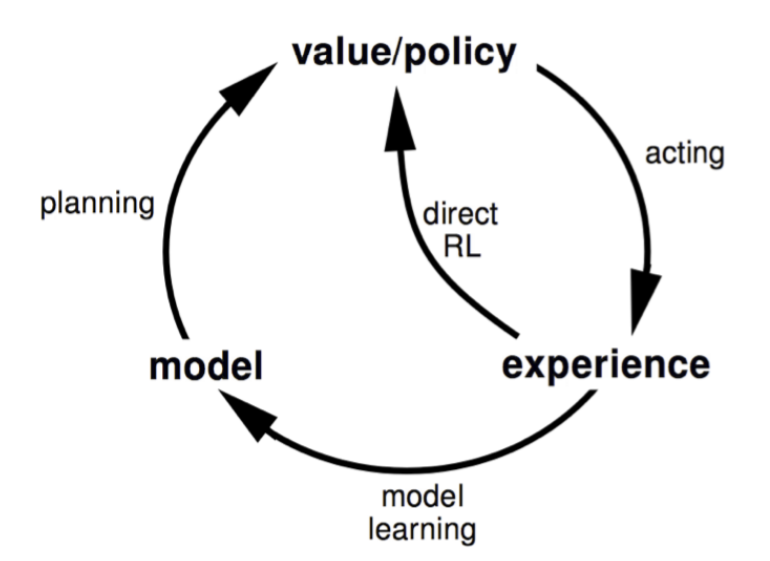
\includegraphics[width=6cm]{dyna}
	\caption{Dyna architecture cycle}
\end{figure}

It is possible to learn and plan the value function (and/or policy) from real and simulated experience. This architecture is referred to as \textbf{Dyna}.The algorithm below uses Dyna with Q-Learning.

\begin{algorithm}[H]
	\caption{Dyna-Q}
	\label{alg:Dyna-Q}
	\begin{algorithmic}
		\REQUIRE $Q$, $M$, $n$ (number of planning steps)
		\STATE $S \Leftarrow$ current state
		\STATE $A \Leftarrow \epsilon$-greedy($S, Q$)
		\STATE Execute $A$; observe $R, S'$
		\STATE $Q(S, A) \Leftarrow Q(S, A) + \alpha \left[R + \gamma \max_a Q(S', a) - Q(S, A)\right]$
		\STATE $M \Leftarrow R,S'$
		\FOR{$i = 1,...,n$}
			\STATE $S, A \Leftarrow$ random previously taken state-action pair
			\STATE $R, S' \Leftarrow M(S, A)$
			\STATE $Q(S, A) \Leftarrow Q(S, A) + \alpha \left[R + \gamma \max_a Q(S', a) - Q(S, A)\right]$
		\ENDFOR
	\end{algorithmic}
\end{algorithm}

Here, the Q-function is learned from both real experience and planned experience.

\section{Simulation-Based Search}

\textbf{Forward search} algorithms select the best action by \textit{lookahead}. They build a search tree with current state $s_t$ at the root. The idea is to use a \textit{model} of the MDP to perform lookahead. Then, only a subsection of the entire MDP must be solved. 

\textbf{Simulation-Based search} simulates episodes of experience from the current state with the model. So, from current state $s_t$, $K$ episodes are sampled:

\begin{equation*}
	\{s_t^k, A_t^k, R_{t+1}^k, ..., S_T^k\}_{k = 1}^K \sim M
\end{equation*}

Then, model-free RL is applied to the simulated episodes. Monte-carlo control gives rise to \textbf{Monte-Carlo search}, while SARSA gives rise to \textbf{TD search}.

Simple Monte-Carlo search uses the mean return to construct Q-values $Q(s_t, a) = \frac{1}{K} \sum_{k = 1}^K G_t$ for each action $a \in A$. This estimates $q_\pi(s_t, a)$, where $\pi$ is the simulation policy. The real action is then taken using $a_t = \arg\max_{a \in A} Q(s_t, a)$.

\subsection{Monte-Carlo Tree Search}

\textbf{Monte-Carlo Tree Search} (MCTS) works differently. It has two policies, a \textit{Tree policy} and a \textit{Default policy}. The tree policy picks the actions to maximize $Q(S, A)$ and the default policy is fixed and takes random actions. So, the tree policy improves over time.

At each simulation, it first uses the tree policy to find with state to simulate from. Then, the simulation (also referred to as rollout) happens using the default policy. The Q-values are then the mean return of episodes.

\begin{equation*}
	Q(s, a) = \frac{1}{N(s, a)} \sum^K_{k = 1} \sum^T_{u = t} 1(S_u, A_u = s, a)G_u
\end{equation*}

After the planning has finished, the real action is again taken using policy $a_t = \arg\max_{a \in A} Q(s_t, a)$. MCTS is MC-control applied to simulated experience. It converges on the optimal search tree, $Q(S, A)$ becomes $q_*(S, A)$.

There are several advantages to using MCTS
\begin{itemize}
	\item The best-first search is highly selective
	\item Evaluates states dynamically, unlike DP
	\item The use of sampling breaks the curse of dimensionality
	\item It works for black-box models, all it needs are samples
	\item Computationally efficient, anytime and parallelisable
\end{itemize}

\subsection{Temporal-Difference Search}

The idea is to use TD instead of MC, by bootstrapping. It applies SARSA to the sub-MDP. It can be helpful for the following reasons
\begin{itemize}
	\item TD search reduces variance, but increases bias
	\item TD search is usually more efficient than MC search
	\item TD($\lambda$) can be much more efficient than MC search
\end{itemize}

\textbf{TD search} simulates episodes from the current state $s_t$. It estimates the value function $Q(S, A)$. At each step of the simulation, $\Delta Q(S, A) = \alpha (R + \gamma Q(S', A') - Q(S, A))$. Actions are selection $\epsilon$-greedily with respect to the Q-values. A function approximator can also be used for Q.

There is another idea called \textbf{Dyna-2}. The agent stores two sets of feature weights: \textit{Long-term memory} and \textit{Short-term (working) memory}. 

The long-term memory is updated from real experience with the environment. It is perceived as general knowledge that applies to any episode. On the other hand, the short-term memory is updated from simulated experience using TD search. This can figure out specific local knowledge about the current situation.

The value function is then a sum of the long- and short-term memories.
